

% Gradient Info
  
\tikzset {_5hbmo8yc4/.code = {\pgfsetadditionalshadetransform{ \pgftransformshift{\pgfpoint{81.84 bp } { -103.62 bp }  }  \pgftransformscale{1.32 }  }}}
\pgfdeclareradialshading{_42co7mn6x}{\pgfpoint{-72bp}{88bp}}{rgb(0bp)=(1,1,1);
rgb(0.052081516810825894bp)=(1,1,1);
rgb(25bp)=(0.74,0.74,0.74);
rgb(400bp)=(0.74,0.74,0.74)}
\tikzset{every picture/.style={line width=0.75pt}} %set default line width to 0.75pt        

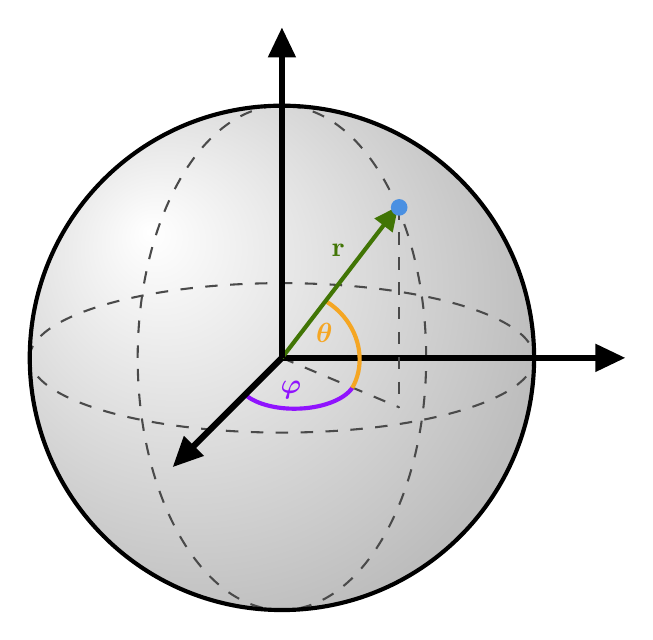
\begin{tikzpicture}[x=0.75pt,y=0.75pt,yscale=-1,xscale=1,style = {font = \boldmath}]
%uncomment if require: \path (0,313); %set diagram left start at 0, and has height of 313

%Shape: Circle [id:dp5460928729364494] 
\draw  [draw opacity=0][shading=_42co7mn6x,_5hbmo8yc4][line width=1.5]  (24,163.5) .. controls (24,96.4) and (78.4,42) .. (145.5,42) .. controls (212.6,42) and (267,96.4) .. (267,163.5) .. controls (267,230.6) and (212.6,285) .. (145.5,285) .. controls (78.4,285) and (24,230.6) .. (24,163.5) -- cycle ;
%Straight Lines [id:da5671603358142259] 
\draw [color={rgb, 255:red, 74; green, 74; blue, 74 }  ,draw opacity=1 ] [dash pattern={on 4.5pt off 4.5pt}]  (145.5,163.5) -- (202,187.33) ;
%Shape: Ellipse [id:dp6506733150555541] 
\draw  [color={rgb, 255:red, 74; green, 74; blue, 74 }  ,draw opacity=1 ][dash pattern={on 4.5pt off 4.5pt}] (76,163.5) .. controls (76,96.4) and (107.12,42) .. (145.5,42) .. controls (183.88,42) and (215,96.4) .. (215,163.5) .. controls (215,230.6) and (183.88,285) .. (145.5,285) .. controls (107.12,285) and (76,230.6) .. (76,163.5) -- cycle ;
%Shape: Ellipse [id:dp26678317589757317] 
\draw  [color={rgb, 255:red, 74; green, 74; blue, 74 }  ,draw opacity=1 ][dash pattern={on 4.5pt off 4.5pt}][line width=0.75]  (24,163.5) .. controls (24,143.62) and (78.4,127.5) .. (145.5,127.5) .. controls (212.6,127.5) and (267,143.62) .. (267,163.5) .. controls (267,183.38) and (212.6,199.5) .. (145.5,199.5) .. controls (78.4,199.5) and (24,183.38) .. (24,163.5) -- cycle ;
%Straight Lines [id:da95744507209868] 
\draw [line width=2.25]    (145.5,163.5) -- (305.8,163.5) ;
\draw [shift={(310.8,163.5)}, rotate = 180] [fill={rgb, 255:red, 0; green, 0; blue, 0 }  ][line width=0.08]  [draw opacity=0] (14.29,-6.86) -- (0,0) -- (14.29,6.86) -- cycle    ;
%Straight Lines [id:da9220607301798066] 
\draw [color={rgb, 255:red, 74; green, 74; blue, 74 }  ,draw opacity=1 ] [dash pattern={on 4.5pt off 4.5pt}]  (202,91) -- (202,187.33) ;
%Shape: Arc [id:dp11613747224217108] 
\draw  [draw opacity=0][line width=1.5]  (179.38,177.98) .. controls (175.34,183.79) and (164.25,188) .. (151.5,188) .. controls (141.03,188) and (132.07,185.16) .. (127.41,180.92) -- (152.5,173.67) -- cycle ; \draw  [color={rgb, 255:red, 144; green, 19; blue, 254 }  ,draw opacity=1 ][line width=1.5]  (179.38,177.98) .. controls (175.34,183.79) and (164.25,188) .. (151.5,188) .. controls (141.03,188) and (132.07,185.16) .. (127.41,180.92) ;
%Shape: Arc [id:dp1998195952216596] 
\draw  [draw opacity=0][line width=1.5]  (166.45,136.09) .. controls (175.38,141.4) and (181.85,150.81) .. (182.82,161.52) .. controls (183.36,167.6) and (182.07,173.26) .. (179.38,177.98) -- (152.82,161.52) -- cycle ; \draw  [color={rgb, 255:red, 245; green, 166; blue, 35 }  ,draw opacity=1 ][line width=1.5]  (166.45,136.09) .. controls (175.38,141.4) and (181.85,150.81) .. (182.82,161.52) .. controls (183.36,167.6) and (182.07,173.26) .. (179.38,177.98) ;
%Straight Lines [id:da3798410950733011] 
\draw [color={rgb, 255:red, 65; green, 117; blue, 5 }  ,draw opacity=1 ][line width=1.5]    (145.5,163.5) -- (199.07,93.67) ;
\draw [shift={(201.5,90.5)}, rotate = 487.49] [fill={rgb, 255:red, 65; green, 117; blue, 5 }  ,fill opacity=1 ][line width=0.08]  [draw opacity=0] (11.61,-5.58) -- (0,0) -- (11.61,5.58) -- cycle    ;
%Shape: Circle [id:dp5016585286703897] 
\draw  [draw opacity=0][fill={rgb, 255:red, 74; green, 144; blue, 226 }  ,fill opacity=1 ] (198,91) .. controls (198,88.79) and (199.79,87) .. (202,87) .. controls (204.21,87) and (206,88.79) .. (206,91) .. controls (206,93.21) and (204.21,95) .. (202,95) .. controls (199.79,95) and (198,93.21) .. (198,91) -- cycle ;
%Straight Lines [id:da5083339397538952] 
\draw [line width=2.25]    (145.5,163.5) -- (96.54,212.46) ;
\draw [shift={(93,216)}, rotate = 315] [fill={rgb, 255:red, 0; green, 0; blue, 0 }  ][line width=0.08]  [draw opacity=0] (14.29,-6.86) -- (0,0) -- (14.29,6.86) -- cycle    ;
%Straight Lines [id:da9550893076013829] 
\draw [line width=2.25]    (145.5,163.5) -- (145.5,9.47) ;
\draw [shift={(145.5,4.47)}, rotate = 450] [fill={rgb, 255:red, 0; green, 0; blue, 0 }  ][line width=0.08]  [draw opacity=0] (14.29,-6.86) -- (0,0) -- (14.29,6.86) -- cycle    ;
%Shape: Circle [id:dp9507399492507013] 
\draw  [line width=1.5]  (24,163.5) .. controls (24,96.4) and (78.4,42) .. (145.5,42) .. controls (212.6,42) and (267,96.4) .. (267,163.5) .. controls (267,230.6) and (212.6,285) .. (145.5,285) .. controls (78.4,285) and (24,230.6) .. (24,163.5) -- cycle ;

% Text Node
\draw (168,107) node [anchor=north west][inner sep=0.75pt]  [color={rgb, 255:red, 65; green, 117; blue, 5 }  ,opacity=1 ] [align=left] {$\displaystyle \mathbf{r}$};
% Text Node
\draw (156.29,184.75) node [anchor=south east] [inner sep=0.75pt]  [color={rgb, 255:red, 144; green, 19; blue, 254 }  ,opacity=1 ] [align=left] {$\displaystyle \mathbf{\varphi }$};
% Text Node
\draw (160.5,145.5) node [anchor=north west][inner sep=0.75pt]  [color={rgb, 255:red, 245; green, 166; blue, 35 }  ,opacity=1 ] [align=left] {$\displaystyle \mathbf{\theta }$};


\end{tikzpicture}
